\section{Evaluation}

\tool is available at \url{flipper.mpi-sws.org}. It consists of a backend
responsible for semantic parsing, a frontend that visually demonstrates to the user the effect of each interpretation of an utterance (both based on \cite{wangVoxelurn}), and a planning module.
%\footnote{The code is available at \url{github/gitlab for both repositories}}.
As our core language is a mixture of concepts typical for
imperative programming (e.g.\ \lstinline{move left}) and an \textit{avoid-until-
reach} temporal specification, we use an adapted version of the
$A^*$~\cite{hipsterHeuristicPlanner} algorithm as our planner. 
% Depending on a deployment scenario and language requirements, we could choose a different
% planner supporting declarative specifications~\cite{metricFF,hadasLTLMop,antlab}.

\subsection{Goal of Evaluation}
Our final goal is to create a system which people with different levels of
proficiency in the core language would use. Envisioned users range from
\emph{expert users}, i.e., those that define new commands to make the
communication with the robot simpler, all the way to those who do not know the
language at all. The latter take advantage of commands that \emph{sound as if they
should work}, and which were defined by other users of the system.

In the evaluation we were thus interested in two properties:
\begin{enumerate}
	\item whether or not users are inclined to define new commands and whether
		those commands make their work easier, and
	\item how much they are able to benefit from other people's definitions
		(without knowing them in advance).
\end{enumerate}
The first property corresponds to the ability to define functions in a programming language,
except that \tool generalizes definitions from examples. The second property
describes how much closer the system gets to pure natural-language interface if
there is a number of active expert users. We thus want to test our intuition
that different people use similar linguistic expressions for similar commands
and that is why they do not have to be aware of existing definitions.

\subsection{Setup}
We created a list of 21 tasks. The tasks levels ranged from easy (e.g.
``get one green square'') to difficult (e.g. ''bring all red items to a
room that contains a yellow square''). The list of all tasks, as well as
all our experimental data is available at \tool's website.
% \todo[inline]{@Ivan: reminder to put list of tasks on website}
%
We recruited thirteen participants, all with prior programming experience but without any
knowledge of the system, and split them into three groups:
\begin{itemize}
	\item Group $A$ (4 members) was only allowed to use the core language,

	\item Group $B$ (6 members) could additionally define their own concepts,

	\item Group $C$ (3 members) additionally had access to concepts defined by two
		expert users (familiar with the system and the language) as well as by other
		participants from group C in real time.
\end{itemize}
%
At the start of the experiment, each group had 30 minutes to familiarize themselves with the core language by following a tutorial. 
%\footnote{tutorial is available at \url{TUTORIALURL}}.
Then participants were instructed to solve the 21 tasks as they saw fit, i.e., not necessarily in the most general way.
The average time needed to solve all tasks was 90 minutes (no deadline was set). 
For each participant, we measured the number of accepted commands, i.e., the syntactically 
correct ones coming either from the core or the induced language,
and the total number of words, defined concepts, and induced commands used to finish all tasks. 
For induced commands we additionally distinguish whether they were defined by the same or by another participant.

%\paragraph*{\textbf{Difficulty of Learning the Core Language}}

Learning any new programming language in half an hour is a nontrivial task. In
our experiment, the average number of successfully parsed queries in group $A$
(only using the core language) was 75\%, with some differences between
the participants (63\%, 70\%, 77\% and 90\%).


\subsection{Results}

\paragraph*{\textbf{Usefulness of Naturalization}}
To assess the usefulness of naturalization, we compare the total number of
tokens needed to finish the tasks for the different groups
(\autoref{fig:numTokens}), and how often participants in groups $B$ and $C$ used
defined concepts (\autoref{fig:groupBAndCCoreVsInduced}).
The latter shows that participants who were allowed to define their own concepts
also used that opportunity.
When comparing the participants from groups $B$ and $C$ to those of group $A$, 
it is clear that the participants who were able to use naturalization end up with less work in 
terms of total number of tokens needed to finish the tasks. 
Specifically, the average number of tokens needed for groups $B$ and $C$ is 1156, 
while for group $A$ it is 1765. 
This takes into account all tokens, also the ones from unsuccessful commands. 
We include these, as some number of unsuccessful commands by groups that use naturalization comes from trying 
out commands they believed might be defined by others.
Only considering successful commands, groups $B$ and $C$ use in total 738 tokens compared to 1287 in group $A$, 
i.e., an improvement of 43\% with respect to the usage of the core language only.
These results suggest that naturalization reduces users' effort. 
It is important to note that individual performances of participants within a single group vary, as shown in~\autoref{fig:numTokens}.

\paragraph*{\textbf{Naturalization across Users}}
Participants in group $C$ had access to the concepts defined by others. Interestingly, these
participants adopted different strategies. While they were on average more likely to use induced
language than the core language (43 vs.\ 35 commands), only one participant relied primarily on the induced language.
The other two users used slightly more core than induced language (see~\autoref{fig:groupBAndCCoreVsInduced}).
The main point of the experiment for group $C$ was to see whether the existence of previously defined concepts is helpful.
We first notice that participants were indeed using concepts defined by others (\autoref{fig:groupCRulesInducedBySelfVsOthers}). 
Again, the numbers differ among participants. 
By looking closer at the kinds of commands issued by each participant, we see that these differences 
stem from their individual styles: participant $C2$ chose to try small building blocks that matched the style of 
the two expert users whose definitions were available to group $C$. 
Participant $C3$, on the other hand, used commands similar to the core language.
%\footnote{All commands by all experiment participants are available at \url{URLFORALLDATA}}.
Curiously, after the experiment two participants (C1 and C3) claimed that they have not much used the predefined rules 
and that they ended up using almost exclusively self-defined concepts (in addition to the the core language). 
The data, however, told a different story (\autoref{fig:groupCRulesInducedBySelfVsOthers}): $C1$ roughly equally used rules defined by others and by himself, while $C3$ 
used much more induced rules. 
Upon inspection of the logs, it turned out that on many occasions they believed they were using the core language, while in fact they used induced concepts
defined by others
(e.g. \lstinline{move 2 right} or \lstinline{drop all blue items}).

\paragraph*{\textbf{Types of Defined Concepts}}
Upon closer inspection of the concepts the participants defined, we see that a majority falls into two categories:
\begin{inparaenum}[(1)]
\item simplifying individual commands and
\item defining functions.
\end{inparaenum}
%
Examples for the first case are
\lstinline{pick green square} defined as \lstinline{pick item has color green} and
\lstinline{visit empty space} defined as \lstinline$visit world minus {world containing item}$.

For the second case a simple example is
\lstinline{visit both triangle and green} defined as
\begin{lstlisting}
visit { {world containing item has shape triangle} and
  {world containing item has color green} }
\end{lstlisting}
There were also function definitions that involved previous function definitions,
such as \lstinline{line red} being defined as
\lstinline$fetch all red; while {robot has item} {drop item; move left}$.
Another noticeable phenomenon was that group C had to define some concepts already defined by others.
The reason was small variations in the utterances (e.g. \lstinline{pick red} vs.\
\lstinline{take a red} vs.\ \lstinline{take a red item}) which can be caught by a more
comprehensive natural language processing module.


\begin{figure}[t!]

		\resizebox{\linewidth}{!}{
		\centering
				\begin{tikzpicture}
				\begin{axis}[
				ticklabel style = {font=\tiny},
				    ybar,
				    bar width = 3,
				    area legend,
				    %enlargelimits=0.15,
				    legend style={at={(0.5,-0.15)},
				      anchor=north,legend columns=-1},
				    ylabel={\# tokens},
				    symbolic x coords={A1, A2, A3, A4, B1,B2,B3,B4,B5,B6,C1,C2,C3},
				    xtick=data,
	%			    nodes near coords,
				    ]
				\addplot coordinates {(A1,1105 ) (A2,1035 ) (A3,1853) (A4, 1156) (B1, 375) (B2, 957) (B3, 549) (B4, 1063) (B5, 970) (B6, 985) (C1,649) (C2,622) (C3,478)};
				\addplot coordinates {(A1,1398 ) (A2,1220 ) (A3,2790) (A4, 1654) (B1, 760) (B2,1364) (B3, 822) (B4, 1471) (B5, 1578) (B6, 1270) (C1,1098) (C2,982) (C3,1061)};
			%	\addplot coordinates {(B1,30) (B2, 61) (B3, 29) (B4, 107) (B5, 80) (B6, 158) (C1,46) (C2,13) (C3,48)};
				\legend{successful commands, all commands}
				\end{axis}
				\end{tikzpicture}
	}
	\caption{Total number of tokens used per participant}
	\label{fig:numTokens}
	\end{figure}






\begin{figure}[t!]
		\resizebox{\linewidth}{!}{
		\centering



				\begin{tikzpicture}
				\begin{axis}[
				    ybar,
				    bar width = 5,
				    area legend,
				    %enlargelimits=0.15,
				    legend style={at={(0.5,-0.15)},
				      anchor=north,legend columns=-1},
				    ylabel={\# commands},
				    symbolic x coords={B1,B2,B3,B4,B5,B6,C1,C2,C3},
				    xtick=data,
	%			    nodes near coords,
				    ]
				\addplot coordinates {(B1, 38) (B2, 64) (B3, 47) (B4, 6) (B5, 45) (B6, 62) (C1,37) (C2,65) (C3,28)};
				\addplot coordinates {(B1,30) (B2, 61) (B3, 29) (B4, 107) (B5, 80) (B6, 158) (C1,46) (C2,13) (C3,48)};
				\legend{induced, core}
				\end{axis}
				\end{tikzpicture}


	}

	\caption{Core-language commands vs induced commands for groups B and C}
	\label{fig:groupBAndCCoreVsInduced}
	\end{figure}


\begin{figure}[t!]
	\resizebox{\linewidth}{!}{
		\centering
		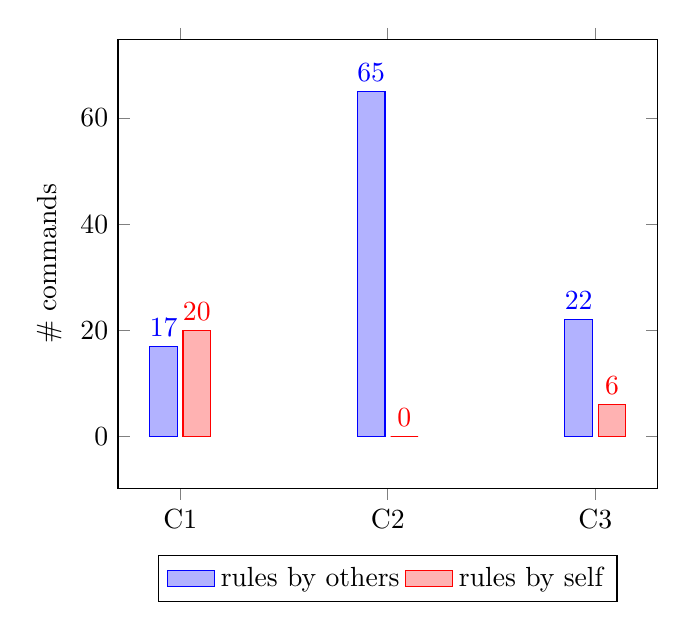
\begin{tikzpicture}
			\begin{axis}[
			    ybar,
			    area legend,
			    enlargelimits=0.15,
			    legend style={at={(0.5,-0.15)},
			      anchor=north,legend columns=-1},
			    ylabel={\# commands},
			    symbolic x coords={C1,C2,C3},
			    xtick=data,
			    nodes near coords,
			    ]
				\addplot coordinates {(C1,17) (C2,65) (C3,22)};
				\addplot coordinates {(C1,20) (C2,0) (C3,6)};
				\legend{rules by others, rules by self}
			\end{axis}
		\end{tikzpicture}
	}
	\caption{Using rules induced by others vs. self-induced rules}
	\label{fig:groupCRulesInducedBySelfVsOthers}
\end{figure}


%\begin{figure}[t!]
%		%\resizebox{\linewidth}{!}{
%		\centering
%		\subfloat[][Core language commands vs induced commands]{\resizebox{0.5\linewidth}{!}{
%
%				\label{fig:groupCCoreVSInduced}
%				\begin{tikzpicture}
%				\begin{axis}[
%				    ybar,
%				    area legend,
%				    enlargelimits=0.15,
%				    legend style={at={(0.5,-0.15)},
%				      anchor=north,legend columns=-1},
%				    ylabel={\# commands},
%				    symbolic x coords={C1,C2,C3},
%				    xtick=data,
%				    nodes near coords,
%				    ]
%				\addplot coordinates {(C1,37) (C2,65) (C3,28)};
%				\addplot coordinates {(C1,46) (C2,13) (C3,48)};
%				\legend{induced, core}
%				\end{axis}
%				\end{tikzpicture}
%
%	}
%			}
%\subfloat[][Using rules induced by others vs. self-induced rules]{\resizebox{0.5\linewidth}{!}{
%
%				\label{fig:groupCRulesInducedBySelfVsOthers}
%				\begin{tikzpicture}
%				\begin{axis}[
%				    ybar,
%				    area legend,
%				    enlargelimits=0.15,
%				    legend style={at={(0.5,-0.15)},
%				      anchor=north,legend columns=-1},
%				    ylabel={\# commands},
%				    symbolic x coords={C1,C2,C3},
%				    xtick=data,
%				    nodes near coords,
%				    ]
%				\addplot coordinates {(C1,17) (C2,65) (C3,22)};
%				\addplot coordinates {(C1,20) (C2,0) (C3,6)};
%				\legend{rules by others, rules by self}
%				\end{axis}
%				\end{tikzpicture}
%
%	}
%			}
%	\caption{Usage of induced rules in group C}
%
%\end{figure}
